\chapter{复杂度治理与目标治理：AgentOS 的双轴运行时治理}
\label{chap:complexity-goal-governance}

在前面的讨论中，工作记忆有限容量定理给出了 AgentOS 最基本的运行约束：任意时刻能够进入全局显式认知表面 $h(t)$ 的有效认知结构是有限的。因此，AgentOS 必须持续回答一个资源问题：

\begin{statementbox}
\centering
\adjustbox{max width=.96\linewidth}{\(\displaystyle \text{当前哪些认知结构应当进入 } h(t)，
\text{以何种形式进入，并占用多少认知资源？}\)}
\end{statementbox}

围绕这一问题，前文逐步形成了 CCM、Scheduler、Boundary 与 Offloading，并将复杂度治理概括为截流、压缩、时序展开、迁移和重构五种基本动作。

然而，仅有复杂度治理仍不足以构成完整的智能治理体系。复杂度治理能够保证系统``做得动''，却不能决定系统``为什么要做''、``应该先做什么''以及``什么时候应该停止做''。一个认知系统完全可能在复杂度受控的情况下，高效地执行一个不重要、已经失效、互相冲突甚至不应被允许的目标。

因此，在复杂度治理之外必须引入一个与之正交但紧密耦合的第二治理维度：

\[
\boxed{
\text{Goal Governance}
}
\]

即目标治理。

本章由此提出 AgentOS 的双轴运行时治理原理：

\[
\boxed{
\text{AgentOS Governance}
=
\text{Complexity Governance}
\bowtie
\text{Goal Governance}
}
\]

复杂度治理管理的是\emph{认知结构如何被承载}；目标治理管理的是\emph{哪些未来约束获得承载资格以及这些未来约束如何相互组织}。前者约束认知系统的运行负荷，后者约束认知系统的方向结构。

二者共同回答：

\[
\boxed{
\text{What should be pursued?}
\quad+\quad
\text{How much cognition should it occupy?}
}
\]

这构成 AgentOS 从``认知资源调度系统''进一步走向``持续自主智能体治理系统''的重要一步。
\begin{figure}[htbp]
\centering
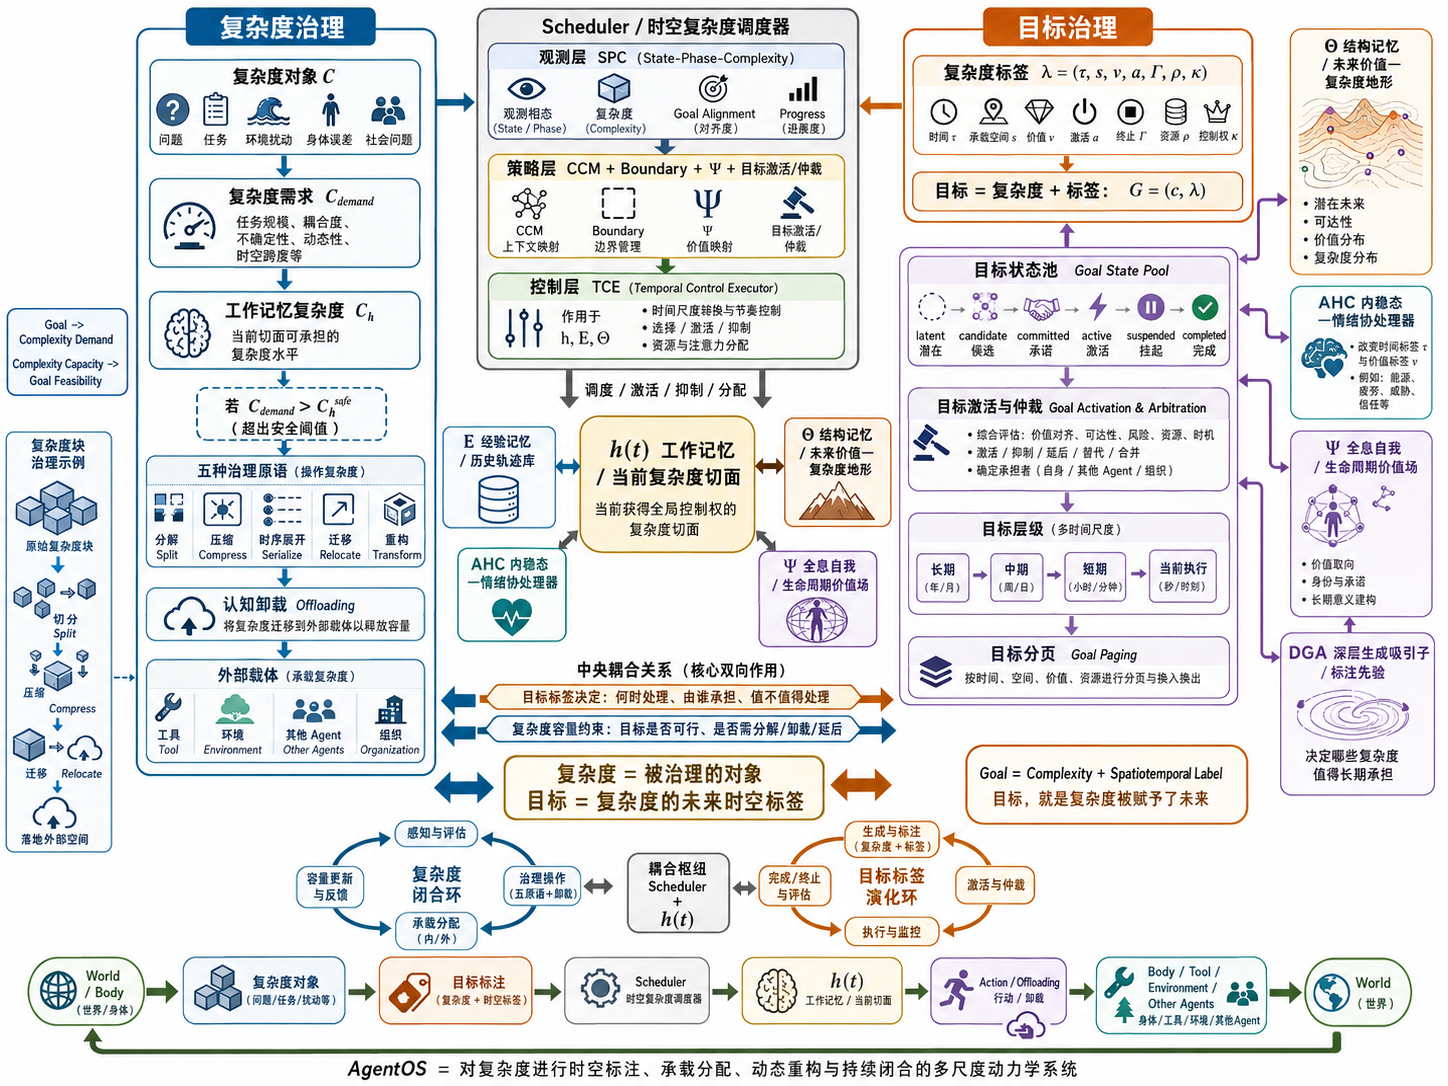
\includegraphics[width=.9\textwidth,height=.38\textheight,keepaspectratio]{images/global-local-predictive-control.png}
\caption{AgentOS的双治理体系区别}
\end{figure}

\section{从有限认知容量到双重治理问题}

工作记忆有限容量定理可以概念性写成：

\[
C_{\mathrm{run}}(t)
\leq
C_{\max}(W),
\]

其中 $C_{\mathrm{run}}(t)$ 表示当前运行态需要由全局认知维持的有效结构负载，$W$ 表示工作记忆有效容量。

这一约束首先产生复杂度治理问题：

\begin{statementbox}
\centering
\adjustbox{max width=.96\linewidth}{\(\displaystyle \text{如何使 }C_{\mathrm{run}}(t)
\leq
C_{\max}(W)?\)}
\end{statementbox}

但进一步观察可以发现，$C_{\mathrm{run}}(t)$ 并不是凭空产生的。大量工作记忆占用来自当前激活的 Goal、Subgoal、Plan、Hypothesis、Constraint 与尚未闭合的 Task。

因此，可以粗略写成：

\[
C_{\mathrm{run}}(t)
=
C_{\mathrm{world}}(t)
+
C_{\mathrm{goal}}(t)
+
C_{\mathrm{plan}}(t)
+
C_{\mathrm{conflict}}(t)
+
C_{\mathrm{coord}}(t),
\]

其中：

\begin{itemize}
    \item $C_{\mathrm{world}}$ 表示当前世界状态和事件带来的结构负载；
    \item $C_{\mathrm{goal}}$ 表示维持活跃 Goal 所需要的认知负载；
    \item $C_{\mathrm{plan}}$ 表示计划、过程与中间状态；
    \item $C_{\mathrm{conflict}}$ 表示多个目标、约束或计划之间的冲突成本；
    \item $C_{\mathrm{coord}}$ 表示维持多个并行过程之间关系所需要的协调成本。
\end{itemize}

这意味着，认知过载不仅可能来自``问题太复杂''，也可能来自：

\begin{statementbox}
\centering
\adjustbox{max width=.96\linewidth}{\(\displaystyle \text{想同时完成的事情太多。}\)}
\end{statementbox}

因此，工作记忆有限性实际上同时推出两个治理问题：

\[
\boxed{
\text{Structure Load Governance}
}
\]

与

\[
\boxed{
\text{Goal Set Governance}.
}
\]

前者就是复杂度治理；后者就是目标治理。

两者不能彼此替代。


\section{复杂度治理与目标治理是两个正交治理平面}

为了区分两个治理对象，可以定义 Agent 在时刻 $t$ 的治理状态：

\[
\boxed{
\mathcal X_{\mathrm{gov}}(t)
=
\left(
\mathcal C_t,
\mathcal G_t
\right),
}
\]

其中 $\mathcal C_t$ 表示当前认知结构负载及其承载状态，$\mathcal G_t$ 表示当前存在的目标结构集合。

复杂度治理作用于：

\[
\mathcal C_t
\longrightarrow
\mathcal C_{t+1},
\]

目标治理作用于：

\[
\mathcal G_t
\longrightarrow
\mathcal G_{t+1}.
\]

两者分别回答：

\[
\boxed{
\text{Complexity Governance: How should cognition be organized?}
}
\]

和：

\[
\boxed{
\text{Goal Governance: Which futures should cognition pursue?}
}
\]

这里必须特别注意，Goal 不等于当前执行动作。Goal 是对未来可接受状态空间的一种约束结构：

\[
\boxed{
G_i
=
\text{Constraint over possible future trajectories}.
}
\]

因此目标治理不是普通任务队列管理。它必须处理：

\[
\text{Goal Generation},
\quad
\text{Goal Admission},
\quad
\text{Goal Priority},
\quad
\text{Goal Commitment},
\quad
\text{Goal Decomposition},
\]

以及：

\[
\text{Goal Suspension},
\quad
\text{Goal Delegation},
\quad
\text{Goal Revision},
\quad
\text{Goal Closure},
\quad
\text{Goal Abortion}.
\]

由此，复杂度治理和目标治理形成两个相互耦合但不可互相化约的治理平面。


\section{目标是未来结构，而不是当前命令}

在简单任务系统中，Goal 往往被表示成一句自然语言：

\[
\texttt{``完成任务 X''}.
\]

但在持续 Agent 中，这种表示远远不够。

一个 Goal 至少应该包含：

\[
\boxed{
G_i
=
\left(
g_i,
\phi_i,
s_i,
a_i,
p_i,
\tau_i,
\mathcal D_i,
\mathcal K_i,
\mathcal V_i,
q_i
\right),
}
\]

其中：

\begin{itemize}
    \item $g_i$：目标语义结构；
    \item $\phi_i$：目标闭合判定条件；
    \item $s_i$：目标来源；
    \item $a_i$：该目标拥有的权限或授权等级；
    \item $p_i$：当前运行优先级；
    \item $\tau_i$：时间尺度、截止时间或有效时间区间；
    \item $\mathcal D_i$：与其他 Goal 的依赖关系；
    \item $\mathcal K_i$：必须满足的约束集合；
    \item $\mathcal V_i$：目标与当前价值、自我和长期方向之间的关系；
    \item $q_i$：当前对目标本身及其可实现性的置信状态。
\end{itemize}

这里尤其重要的是 $\phi_i$。

没有显式闭合条件的 Goal 很容易形成：

\[
\boxed{
Never-Ending Cognitive Process.
}
\]

例如``继续研究''、``继续优化''、``继续寻找更好的方案''都可能无限占用认知资源。

因此一个成熟的目标治理系统不仅必须能够产生 Goal，还必须能够回答：

\[
\boxed{
\text{When is this goal actually finished?}
}
\]

Goal Closure 与 Goal Generation 同等重要。


\section{目标并不是价值本身}

在后续生命周期理论中已经存在：

\[
\Psi
\]

和

\[
\Omega\equiv DGA.
\]

因此必须严格避免将 Goal、Value、Self 与 DGA 混为一谈。

可以区分：

\[
\boxed{
G:\text{What future state is currently pursued?}
}
\]

\[
\boxed{
\Psi:\text{Who am I and what structures should remain self-consistent?}
}
\]

\[
\boxed{
\Omega:\text{What am I becoming over the lifecycle?}
}
\]

Goal 是相对快速的未来约束；$\Psi$ 是更慢的身份与价值约束；$\Omega$ 是更慢的生命周期生成方向。

因此：

\[
\tau_G
\ll
\tau_\Psi
\ll
\tau_\Omega
\]

在典型情况下成立。

这意味着 Goal 可以频繁产生和关闭，而 $\Psi$ 与 $\Omega$ 不应随每一个短期 Goal 同步改变。

更准确地说：

\[
\boxed{
\Psi,\Omega
\rightarrow
GoalFeasibleRegion
}
\]

而不是：

\begin{statementbox}
\centering
\adjustbox{max width=.96\linewidth}{\(\displaystyle Goal
\rightarrow
\Psi,\Omega
\quad\text{immediately}.\)}
\end{statementbox}

慢变量定义目标可以活动的长期区域；短期目标在这一约束区域中获得局部自由度。


\section{目标候选的来源}

持续 Agent 的目标不应只有一个外部输入来源。

可以定义目标候选集合：

\[
\mathcal G^{\mathrm{candidate}}_t
=
\mathcal G^{\mathrm{external}}_t
\cup
\mathcal G^{\mathrm{internal}}_t
\cup
\mathcal G^{\mathrm{maintenance}}_t
\cup
\mathcal G^{\mathrm{derived}}_t.
\]

其中：

外部目标来自用户、组织、环境任务或显式指令；

内部目标来自 Agent 当前 Goal 的进一步推导；

维护目标来自系统稳定、自我维持、恢复、记忆整理等内部需求；

派生目标则是为实现更高层 Goal 自动产生的 Subgoal。

例如：

\[
G_{\mathrm{build}}
\]

可能自动生成：

\[
G_{\mathrm{find\ material}},
\quad
G_{\mathrm{plan}},
\quad
G_{\mathrm{execute}},
\quad
G_{\mathrm{verify}}.
\]

因此：

\[
\boxed{
GoalGeneration
\neq
GoalAdmission.
}
\]

一个 Goal 能够被生成，并不意味着它必然能够进入 Agent 的有效目标集合。


\section{目标准入：并非所有目标都拥有执行资格}

与复杂度治理中的``截流''对应，目标治理首先需要：

\[
\boxed{
Goal Admission.
}
\]

定义候选 Goal：

\[
G_i\in\mathcal G^{\mathrm{candidate}}.
\]

经过治理后：

\[
G_i
\longrightarrow
\begin{cases}
\mathcal G^{\mathrm{admitted}},\\
\mathcal G^{\mathrm{deferred}},\\
\mathcal G^{\mathrm{rejected}}.
\end{cases}
\]

准入不能只根据当前优先级决定，还必须至少考虑：

\[
Authority,
\quad
Safety,
\quad
SelfConsistency,
\quad
LongTermDirection,
\]

\[
Feasibility,
\quad
Cost,
\quad
Risk,
\quad
Conflict,
\quad
RealityConditions.
\]

因此可以概念性定义：

\[
A_G(G_i)
=
F(
Authority_i,
Safety_i,
\Psi_i,
\Omega_i,
Feasibility_i,
Risk_i,
Conflict_i
).
\]

只有：

\[
A_G(G_i)\in\mathcal A_{\mathrm{admissible}}
\]

时，Goal 才进入正式治理集合。

这里体现一个非常重要的 AgentOS 原则：

\[
\boxed{
GoalGeneration
\neq
GoalAuthority.
}
\]

Agent 能够想到一个目标，不意味着它拥有执行这个目标的权限。


\section{目标优先级不应退化为单一效用函数}

最简单的 Goal Scheduler 可以构造：

\[
Score(G_i)
=
w_1U_i
+
w_2Urgency_i
+
w_3Importance_i
-
w_4Risk_i
-
w_5Cost_i.
\]

这种标量化在工程实现中可能有用，但它不应成为目标治理的本体定义。

因为现实中的 Goal 往往同时受到：

\[
Safety,
\quad
Authority,
\quad
Identity,
\quad
Time,
\quad
Resource,
\quad
SocialConstraint
\]

等不同维度约束。

这些约束并不总能被合理压缩成同一个数字。

因此，更一般的目标选择问题应该写成：

\[
\boxed{
G^*
\in
\operatorname{Select}
\left(
\mathcal G_{\mathrm{admitted}}
\mid
\mathcal K_{\mathrm{hard}},
\mathcal V_{\mathrm{soft}}
\right),
}
\]

其中 $\mathcal K_{\mathrm{hard}}$ 表示不可违反的硬约束，$\mathcal V_{\mathrm{soft}}$ 表示可以权衡的软偏好。

由此形成：

\[
\boxed{
Constraint First,\ Preference Second.
}
\]

这比把整个 AgentOS 压缩成一个单一 reward maximizer 更符合持续主体的治理结构。


\section{目标承诺与目标注意是两个不同概念}

一个被 Agent 接受的长期 Goal，并不意味着它必须持续占据 $h(t)$。

因此必须区分：

\[
\boxed{
GoalCommitment
}
\]

和：

\[
\boxed{
GoalActivation.
}
\]

某个 Goal 可以处于长期 committed 状态：

\[
G_i\in\mathcal G^{\mathrm{committed}}
\]

但当前并不活跃：

\[
G_i\notin\mathcal G_h(t).
\]

只有当 Scheduler 判断：

\[
Activate(G_i,t)=1
\]

时，它才被提升到当前认知表面。

因此：

\[
\boxed{
CommittedGoal
\neq
WorkingMemoryResidentGoal.
}
\]

这一设计极其重要。

否则一个拥有大量长期目标的 Agent 会因为试图同时显式维持所有目标而立即违反工作记忆有限容量定理。

成熟 Agent 应当拥有：

\[
\boxed{
ManyPersistentGoals
+
FewActiveGoals.
}
\]


\section{目标并发本身也是一种认知负载}

设当前进入工作记忆的目标集合为：

\[
\mathcal G_h(t)
=
\{G_1,\dots,G_n\}.
\]

每个目标需要维持的结构负载为：

\[
c_i(t).
\]

则：

\[
C_G(t)
=
\sum_{i=1}^{n}
w_i(t)c_i(t).
\]

但多个 Goal 之间还可能产生冲突。

定义目标冲突函数：

\[
\chi(G_i,G_j)
\geq0.
\]

则目标冲突负载可以概念性表示为：

\[
C_{\mathrm{goal-conflict}}(t)
=
\sum_{i\neq j}
w_iw_j
\chi(G_i,G_j).
\]

于是：

\[
\boxed{
C_{\mathrm{goal}}
=
C_{\mathrm{individual}}
+
C_{\mathrm{goal-conflict}}.
}
\]

这说明：

十个各自很简单的目标，

可能比一个复杂目标产生更大的工作记忆压力。

因此复杂度治理与目标治理发生直接耦合：

\begin{statementbox}
\centering
\adjustbox{max width=.96\linewidth}{\(\displaystyle GoalSet
\rightarrow
CognitiveLoad.\)}
\end{statementbox}

反过来：

\begin{statementbox}
\centering
\adjustbox{max width=.96\linewidth}{\(\displaystyle CognitiveCapacity
\rightarrow
AllowedGoalConcurrency.\)}
\end{statementbox}

二者形成闭环，而不是上下级关系。


\section{复杂度治理的五种基本动作}

在此前理论中，复杂度治理形成了五种最基本动作：

\[
\boxed{
\mathcal O_C
=
\{
Cut,
Compress,
Temporalize,
Migrate,
Reorganize
\}.
}
\]

对应中文分别为：

\begin{statementbox}
\centering
\adjustbox{max width=.96\linewidth}{\(\displaystyle 截流、压缩、时序展开、迁移、重构。\)}
\end{statementbox}

截流解决的是：

\begin{statementbox}
\centering
\adjustbox{max width=.96\linewidth}{\(\displaystyle \text{哪些结构根本不应进入 }h.\)}
\end{statementbox}

压缩解决：

\[
X
\rightarrow
\widetilde X,
\qquad
C(\widetilde X)<C(X),
\]

同时尽量保持当前 Goal 所需要的信息。

时序展开解决：

\[
C_{\mathrm{parallel}}
\rightarrow
C_{\mathrm{serial}},
\]

将无法同时承担的空间并发负荷转换成多个时间阶段。

迁移解决：

\[
AgentCSO@Carrier_i
\rightarrow
AgentCSO@Carrier_j,
\]

例如从 $h$ 迁入 $E$、Skill、Tool、File、Environment 或 Other Agent。

重构解决的是：

\[
Representation_i
\rightarrow
Representation_j,
\]

通过改变问题表达、任务分解、约束结构甚至外部环境，使原本难以承载的问题进入新的可解结构。


\section{与复杂度治理并列的五种目标治理动作}

目标治理可以形成一组与上述结构近似平行的基本操作：

\[
\boxed{
\mathcal O_G
=
\{
Admit,
Abstract,
Stage,
Delegate,
Reframe
\}.
}
\]

分别可以译为：

\begin{statementbox}
\centering
\adjustbox{max width=.96\linewidth}{\(\displaystyle 准入、聚合、阶段化、委派、重解释。\)}
\end{statementbox}

它们与复杂度治理存在结构对应关系：

\[
\begin{array}{c|c}
\text{Complexity Governance}
&
\text{Goal Governance}
\\
\hline
\text{截流}
&
\text{目标准入}
\\
\text{压缩}
&
\text{目标聚合/抽象}
\\
\text{时序展开}
&
\text{目标阶段化}
\\
\text{迁移}
&
\text{目标委派}
\\
\text{重构}
&
\text{目标重解释}
\end{array}
\]

但这种对应并不是一一相同的算法，而是两个治理平面具有类似结构。


\section{目标准入：控制未来约束进入主体}

目标准入回答：

\[
\boxed{
Should this future become one of my futures?
}
\]

外部请求、内部欲求、预测风险和派生 Subgoal 都首先只是 candidate。

经过 Authority、Safety、$\Psi$、$\Omega$、现实可行性和资源约束以后，才可能变成正式 Goal。

因此：

\[
CandidateGoal
\rightarrow
AdmittedGoal
\]

是目标治理最基本的边界动作。

复杂度治理中的截流保护的是：

\[
h
\]

目标治理中的准入保护的则是：

\[
\boxed{
AgentFutureSpace.
}
\]


\section{目标聚合：减少碎片化未来}

多个具体目标可能实际上属于一个更高层目标：

\[
G_1,G_2,\dots,G_n
\rightarrow
G_{\mathrm{abstract}}.
\]

例如：

\[
\text{整理文件},
\quad
\text{回复邮件},
\quad
\text{更新计划}
\]

可能共同属于：

\[
\text{完成今日工作收尾}.
\]

这种操作不是简单删除 Goal，而是发现：

\[
\boxed{
SharedHigherOrderConstraint.
}
\]

目标聚合可以显著降低：

\[
C_{\mathrm{coord}}
\]

和：

\[
C_{\mathrm{goal-conflict}}.
\]

因此目标抽象本身也是降低认知复杂度的重要机制。


\section{目标阶段化：把同时未来变成有顺序的未来}

当多个 Goal 无法同时进入 $h$ 时，可以进行：

\[
\boxed{
GoalTemporalization.
}
\]

例如：

\[
\{G_1,G_2,G_3,G_4\}
\]

被重新组织成：

\[
G_1
\rightarrow
G_2
\rightarrow
G_3
\rightarrow
G_4.
\]

复杂度治理称之为时序展开；

目标治理则体现为：

\[
\boxed{
GoalStaging.
}
\]

这表明时间本身是一种认知治理资源。

有限工作记忆并不意味着 Agent 无法完成高复杂度任务，而意味着：

\begin{statementbox}
\centering
\adjustbox{max width=.96\linewidth}{\(\displaystyle \text{很多复杂问题必须通过时间展开才能被有限主体完成。}\)}
\end{statementbox}


\section{目标委派：把未来约束交给其他载体}

复杂度迁移对应的是认知结构改变载体。

目标治理中则存在：

\[
\boxed{
GoalDelegation.
}
\]

例如：

\[
G_A
\rightarrow
G_{\mathrm{tool}},
\]

或者：

\[
G_A
\rightarrow
G_B,
\]

表示 Agent 将某一子目标交由 Tool、External Process 或 Other Agent 完成。

但目标委派并不等于目标责任完全消失。

如果 Agent 仍然是上层 Goal 的承诺主体，则必须保留：

\[
\boxed{
VerificationResponsibility.
}
\]

因此：

\[
Delegate(G_i)
\neq
Forget(G_i).
\]

更准确地：

\begin{statementbox}
\centering
\adjustbox{max width=.96\linewidth}{\(\displaystyle ExecutionAuthority
\rightarrow
ExternalCarrier,
\qquad
ClosureAuthority
\ \text{may remain internal}.\)}
\end{statementbox}

这为后续 Agent 间协作和组织智能提供了重要基础。


\section{目标重解释：改变问题，而不仅是继续执行问题}

有时一个 Goal 长期无法实现，不是因为执行能力不足，而是目标本身的表达结构有问题。

例如原目标：

\[
G:
\text{找到唯一正确答案}
\]

可能被重新解释为：

\[
G':
\text{找到满足当前约束的可行答案}.
\]

这种变化可以写成：

\[
\boxed{
G
\rightarrow
G'
}
\]

而不是简单修改 Plan。

它对应复杂度治理中的 Representation Reorganization。

目标重解释尤其依赖：

\[
RealityFeedback,
\quad
\Psi,
\quad
\Omega,
\quad
Experience.
\]

因此，它不能被普通 Task Scheduler 随意执行，而应具有更高治理门槛。


\section{目标的生命周期状态机}

除了五种基本转换动作，目标治理还必须拥有完整生命周期。

定义：

\[
State(G_i)
\in
\{
Proposed,
Admitted,
Committed,
Active,
Suspended,
Delegated,
Achieved,
Failed,
Aborted,
Superseded
\}.
\]

典型过程为：

\[
Proposed
\rightarrow
Admitted
\rightarrow
Committed
\rightarrow
Active.
\]

执行以后可以进入：

\[
Active
\rightarrow
Achieved,
\]

或：

\[
Active
\rightarrow
Failed,
\]

也可能：

\[
Active
\rightarrow
Suspended,
\]

随后重新：

\[
Suspended
\rightarrow
Active.
\]

如果 Goal 已经失去意义：

\[
Active
\rightarrow
Aborted.
\]

如果更高质量的新 Goal 替代旧 Goal：

\[
G_i
\rightarrow
G_j,
\qquad
State(G_i)=Superseded.
\]

这一状态机使 Goal 从一句 Prompt 变成真正具有生命周期的系统对象。


\section{目标闭合是智能持续运行的必要条件}

一个长期 Agent 最大的潜在问题之一不是无法产生 Goal，而是无法关闭 Goal。

如果：

\[
GenerationRate_G
>
ClosureRate_G
\]

长期成立，则：

\[
|\mathcal G_{\mathrm{open}}|
\rightarrow
\infty.
\]

即使每个 Goal 本身很简单，未闭合 Goal 仍然会不断积累：

Reminder；

Dependency；

Uncertainty；

Pending Verification；

Future Commitment。

因此可以定义 Goal Backlog：

\[
B_G(t)
=
|\mathcal G_{\mathrm{open}}(t)|.
\]

成熟系统必须保证在长期尺度上：

\[
\boxed{
\mathbb E[
GenerationRate_G
]
\lesssim
\mathbb E[
ClosureRate_G
]
}
\]

或者通过：

Abortion；

Aggregation；

Delegation；

Archival；

Reinterpretation

避免目标集合无限增长。

这与内存系统中垃圾回收存在一定工程类比：

\[
\boxed{
GoalGovernance
\text{ requires semantic closure and garbage collection.}
}
\]

但 Goal Closure 比普通对象回收更加复杂，因为目标可能涉及承诺、权限、外部责任和生命周期意义。


\section{Goal Closure 必须通过现实验证}

目标闭合不能仅由 Agent 内部判断：

\[
\boxed{
InternalBelief(G_i=Done)
\not\Rightarrow
G_i=Done.
}
\]

应由闭合条件：

\[
\phi_i
\]

结合可获得的现实证据进行验证：

\[
\boxed{
Closure(G_i)
=
Verify(
\phi_i,
Observation,
ExternalEvidence
).
}
\]

因此：

\[
ActionIssued
\neq
GoalAchieved.
\]

同样：

\[
PlanCompleted
\neq
GoalAchieved.
\]

更不能：

\[
SelfReportedSuccess
=
RealitySuccess.
\]

这与全书的基本原则一致：

\[
\boxed{
RealityIsUltimateConstraint.
}
\]

目标治理最终必须回到现实闭环，而不是形成纯内部语义自证。


\section{目标冲突不仅是优先级冲突}

两个 Goal 之间至少可能存在四种关系：

\[
\boxed{
Independent,
Supporting,
Competing,
Contradictory.
}
\]

独立 Goal 可以并行；

支持型 Goal 可以形成共同结构；

竞争型 Goal 争夺有限资源；

矛盾型 Goal 则无法在相同约束下同时满足。

定义：

\[
R_G(G_i,G_j)
\in
\{
Independent,
Support,
Competition,
Contradiction
\}.
\]

因此目标治理不应只保存 Goal List，还应维护：

\[
\boxed{
GoalGraph.
}
\]

可以写成：

\[
\mathcal G_G
=
(V_G,E_G),
\]

其中节点是 Goal，边表示：

Dependency；

Support；

Conflict；

Exclusion；

TemporalOrder；

Delegation；

Subgoal

等关系。

于是复杂目标规划实际上形成：

\begin{statementbox}
\centering
\adjustbox{max width=.96\linewidth}{\(\displaystyle GoalGraph
\rightarrow
ProcessGraph
\rightarrow
Action.\)}
\end{statementbox}

目标治理因而与前文 CSO 图理论天然兼容：Goal 本身就是一种特殊 CSO。


\section{目标治理与 Scheduler 的关系}

Scheduler 并不等于 Goal Governance。

目标治理决定：

\[
\boxed{
What may deserve pursuit?
}
\]

Scheduler 决定：

\[
\boxed{
What should receive resources now?
}
\]

因此：

\[
GoalGovernance
\rightarrow
EligibleGoalSet
\]

而：

\[
Scheduler
:
EligibleGoalSet
\rightarrow
ActiveGoalSet(t).
\]

可以写成：

\[
\mathcal G_{\mathrm{candidate}}
\xrightarrow{\mathrm{Governance}}
\mathcal G_{\mathrm{eligible}}
\xrightarrow{\mathrm{Scheduler}}
\mathcal G_h(t).
\]

这一区分非常重要。

否则 Scheduler 会被赋予不应拥有的权限：它不仅决定何时执行 Goal，还隐式决定什么值得成为 Goal。


\section{目标治理与 CCM 的关系}

CCM 负责保证：

\[
C_{\mathrm{run}}(t)
\le
C_{\max}.
\]

目标治理则管理：

\[
\mathcal G_t.
\]

二者交互形成：

\[
\boxed{
\mathcal G_t
\rightarrow
C_{\mathrm{run}}
\rightarrow
CCM
\rightarrow
GoalActivation/Decomposition/Staging.
}
\]

如果某一 Goal 需要：

\[
C(G_i)
>
C_{\max},
\]

并不意味着该 Goal 必须被拒绝。

CCM 可以要求目标治理对它进行：

\[
G_i
\rightarrow
\{g_{i1},g_{i2},\dots,g_{in}\}
\]

然后：

\[
C(g_{ik})
<
C_{\max}.
\]

于是：

\[
\boxed{
GoalDecomposition
}
\]

成为连接目标治理和复杂度治理的重要桥梁。

可以概括为：

\[
\boxed{
GoalGovernance
\text{ decides what future matters;}
}
\]

\[
\boxed{
CCM
\text{ decides how that future becomes cognitively tractable.}
}
\]


\section{目标治理与 Boundary 的关系}

Boundary 原本决定：

什么进入认知系统；

什么停留外部；

什么被延迟；

什么被忽略。

从目标治理角度，Boundary 还必须决定：

\begin{statementbox}
\centering
\adjustbox{max width=.96\linewidth}{\(\displaystyle \text{哪些外部要求有资格成为内部承诺。}\)}
\end{statementbox}

例如：

ExternalRequest

并不自动等于：

InternalGoal。

必须经过：

\[
ExternalRequest
\xrightarrow{Boundary}
CandidateGoal
\xrightarrow{Governance}
CommittedGoal.
\]

因此：

\[
\boxed{
CommandReceived
\neq
GoalAccepted.
}
\]

这一原则对长期自主 Agent 极其重要。

否则 Agent 实际上没有认知边界，而只是一个永久接受外部 Goal 注入的执行器。


\section{目标治理与 SPC--TCE 的关系}

SPC 可以观察的不仅是：

CognitiveLoad，

还包括：

GoalConflict；

GoalPersistence；

GoalClosureRate；

UnresolvedGoalPressure；

SelfConsistency；

GoalProgress。

因此 SPC 的自状态估计可以扩展为：

\[
S_{\mathrm{self}}
=
SPC(
h,
\mathcal G,
E,
\Psi,
\ldots
).
\]

TCE 则可以依据 Goal 状态调整：

探索；

搜索深度；

认知温度；

注意持续时间；

资源投入。

例如高价值但低置信 Goal 可能需要：

\[
Exploration\uparrow,
\]

而已接近闭合的 Goal 可能需要：

\[
Convergence\uparrow.
\]

因此：

\begin{statementbox}
\centering
\adjustbox{max width=.96\linewidth}{\(\displaystyle GoalGovernance
\rightarrow
TCEOperatingRegime.\)}
\end{statementbox}

但 TCE 仍然只是调节认知动力学，不拥有创建、修改或授权高层 Goal 的最终治理权。


\section{目标治理与自我 $\Psi$}

长期 Agent 不能只拥有 Goal，还必须拥有 Goal 与 Self 的关系。

定义：

\[
S_\Psi(G_i)
=
Consistency(G_i,\Psi).
\]

它不应被理解成：

\[
S_\Psi=1
\Rightarrow
GoalAccepted.
\]

而应作为目标治理的一个慢约束变量。

因为完全由 $\Psi$ 排斥与当前自我不一致的 Goal，会导致：

\[
\boxed{
IdentityLockIn.
}
\]

Agent 将失去成长能力。

相反，如果任何短期 Goal 都可以迅速改写 $\Psi$，则产生：

\[
\boxed{
IdentityDrift.
}
\]

因此理想结构应为：

\[
\boxed{
Goal
\leftrightarrow
\Psi
}
\]

但具有明显时间尺度分离：

\[
\tau_G
\ll
\tau_\Psi.
\]

Goal 在 Self 所定义的宽约束区间中活动；只有大量长期、稳定、现实验证过的经历，才可能反向缓慢改变 $\Psi$。


\section{目标治理与 DGA/$\Omega$}

如果 $\Psi$ 回答：

\[
WhoAmI,
\]

那么 $\Omega$ 更多描述：

\[
WhatAmIBecoming.
\]

因此可以定义：

\[
S_\Omega(G_i)
=
DevelopmentalCompatibility(G_i,\Omega).
\]

长期目标治理不能只考虑：

\[
ImmediateUtility.
\]

还要考虑：

\[
\boxed{
LongTermDevelopmentalEffect.
}
\]

一个短期 Goal 可能立即有益，却持续把 Agent 引向与生命周期长期方向冲突的状态空间。

因此未来更完整的 Goal Governance 应比较：

\[
ImmediateOutcome
\]

和：

\[
EffectOnFutureSelf.
\]

即：

\[
G_i
\rightarrow
Experience_i
\rightarrow
\Theta'
\rightarrow
\Psi'
\rightarrow
FutureAgent.
\]

目标治理由此第一次与后续的 Agent 培育工程发生直接连接。


\section{目标治理不能形成自我封闭价值系统}

随着 $\Psi$ 和 $\Omega$ 被引入，一个危险是：

\[
Goal
\rightarrow
SelfInterpretation
\rightarrow
Goal
\]

形成封闭循环。

例如：

\[
\Psi
\Rightarrow
G
\Rightarrow
SelectiveObservation
\Rightarrow
Evidence
\Rightarrow
\Psi'.
\]

如果现实反证被持续过滤，系统可能形成内部完全一致、但现实完全错误的目标体系。

因此必须加入：

\[
\boxed{
WorldVerification.
}
\]

任何长期目标结构都应允许：

\[
ExternalEvidence
\rightarrow
GoalRevision,
\]

甚至：

\[
ExternalEvidence
\rightarrow
GoalAbortion.
\]

因此：

\[
\boxed{
SelfConsistency
\neq
Truth.
}
\]

以及：

\[
\boxed{
GoalPersistence
\neq
GoalCorrectness.
}
\]

这也是 AgentOS 长期认知稳定性的根本原则之一。


\section{复杂度治理与目标治理的耦合动力学}

现在可以将两类治理写成一个联合系统。

设：

\[
\mathcal C(t)
\]

为当前认知负载结构，

\[
\mathcal G(t)
\]

为当前目标图。

则：

\[
\dot{\mathcal C}
=
F_C(
\mathcal C,
\mathcal G,
u_C,
W
),
\]

\[
\dot{\mathcal G}
=
F_G(
\mathcal G,
Reality,
\Psi,
\Omega,
u_G
),
\]

其中 $u_C$ 是复杂度治理动作，$u_G$ 是目标治理动作。

二者交叉耦合：

\[
\frac{\partial F_C}{\partial \mathcal G}
\neq0,
\]

因为目标集合改变认知负载；

同时：

\[
\frac{\partial F_G}{\partial \mathcal C}
\neq0,
\]

因为当前认知能力决定哪些目标能够被同时展开和处理。

因此：

\[
\boxed{
ComplexityGovernance
\bowtie
GoalGovernance
}
\]

是一个真实的双向耦合系统。


\section{双轴治理的可行区域}

可以定义 AgentOS 当前的可运行区域：

\[
\boxed{
\mathcal F_{\mathrm{Agent}}
=
\mathcal F_C
\cap
\mathcal F_G
\cap
\mathcal F_A
\cap
\mathcal F_S
\cap
\mathcal F_R,
}
\]

其中：

\[
\mathcal F_C:
C_{\mathrm{run}}
\le
C_{\max},
\]

表示认知容量约束；

\[
\mathcal F_G
\]

表示目标之间不存在不可治理矛盾；

\[
\mathcal F_A
\]

表示 Authority 允许；

\[
\mathcal F_S
\]

表示 Safety 允许；

\[
\mathcal F_R
\]

表示现实可行。

因此 Agent 的决策不应理解成：

\[
\max Reward,
\]

而更一般地是：

\begin{statementbox}
\centering
\adjustbox{max width=.96\linewidth}{\(\displaystyle \text{在可行治理区域中寻找可接受未来轨迹。}\)}
\end{statementbox}

可以写成：

\[
\pi_t
\in
\Pi_{\mathrm{feasible}}
\]

其中：

\[
\Pi_{\mathrm{feasible}}
=
\Pi_C
\cap
\Pi_G
\cap
\Pi_A
\cap
\Pi_S
\cap
\Pi_R.
\]

这为后续将 AgentOS 与约束优化、最优控制和多目标决策连接提供了数学入口。


\section{目标治理也存在快慢时间尺度}

并非所有 Goal 都位于相同时间尺度。

可以粗略划分：

\[
G^{fast},
\quad
G^{task},
\quad
G^{strategic},
\quad
G^{lifecycle}.
\]

对应：

即时行动目标；

任务目标；

战略目标；

生命周期目标。

因此：

\[
\tau_{G^{fast}}
<
\tau_{G^{task}}
<
\tau_{G^{strategic}}
<
\tau_{G^{lifecycle}}.
\]

快 Goal 应当服从慢 Goal 的可行域约束：

\begin{statementbox}
\centering
\adjustbox{max width=.96\linewidth}{\(\displaystyle SlowGoal
\rightarrow
FeasibleRegion(FastGoal).\)}
\end{statementbox}

但慢 Goal 不应逐步控制每个快动作：

\[
\boxed{
SlowGovernance
\neq
FastMicromanagement.
}
\]

这与全书多尺度动力学的基本原则完全一致。


\section{目标层级不是简单树，而是动态目标图}

传统 Planning 常将 Goal 分解为一棵树：

\[
G
\rightarrow
g_1,g_2,\dots,g_n.
\]

对于持续 Agent，这通常不够。

因为一个 Subgoal 可能同时服务于多个高层 Goal；

两个 Goal 可能共享约束；

Goal 之间可能动态竞争、合并或替代。

因此更一般地：

\[
\boxed{
GoalStructure
=
DynamicGoalGraph.
}
\]

图中的边可以表示：

\[
DependsOn,
\quad
Supports,
\quad
ConflictsWith,
\quad
Excludes,
\]

\[
Precedes,
\quad
DelegatesTo,
\quad
Abstracts,
\quad
Supersedes.
\]

这使目标治理自然成为 CSO 图理论的一个特殊子结构：

\[
\boxed{
\mathcal G_G
\subset
\mathcal G_C.
}
\]

Goal 不是 AgentOS 之外附加的一种任务语言，而是 CSO 世界中特殊的未来约束型结构。


\section{复杂度治理与目标治理共同产生过程治理}

Goal 决定：

\[
FutureConstraint,
\]

Complexity Governance 决定：

\[
CognitiveFeasibility.
\]

两者结合产生：

\[
\boxed{
Process.
}
\]

可以写：

\[
Goal
+
CurrentState
+
CapacityConstraint
\rightarrow
Process.
\]

Process 再产生：

\[
Plan,
\quad
Subgoal,
\quad
Action,
\quad
Verification.
\]

因此：

\begin{statementbox}
\centering
\adjustbox{max width=.96\linewidth}{\(\displaystyle Goal
\rightarrow
Process
\rightarrow
Action
\rightarrow
Verify
\rightarrow
Closure\)}
\end{statementbox}

构成此前 L4 Goal--Process 闭环的理论来源。

这说明 Process 并不是 Goal 本身，也不是 Complexity 本身，而是：

\begin{statementbox}
\centering
\adjustbox{max width=.96\linewidth}{\(\displaystyle \text{目标结构在有限认知容量和现实约束下的可执行展开。}\)}
\end{statementbox}


\section{从双轴治理到 AgentOS 的运行时总循环}

至此可以得到一个比单纯：

\[
SPC
\rightarrow
Scheduler
\rightarrow
TCE
\rightarrow
CCM
\]

更完整的治理循环。

首先形成目标候选：

\[
World/Self/Task
\rightarrow
GoalCandidate.
\]

随后：

\[
GoalCandidate
\xrightarrow{
Boundary,\ Authority,\Psi,\Omega
}
EligibleGoal.
\]

Scheduler 决定：

\[
EligibleGoal
\rightarrow
ActiveGoal.
\]

CCM 判断：

\[
ActiveGoal
+
CurrentStructure
\rightarrow
CognitiveFeasibility.
\]

如果复杂度过高：

\[
Decompose,
Compress,
Stage,
Delegate,
Reframe.
\]

随后：

\[
SPC
\rightarrow
TCE
\rightarrow
CognitiveDynamics.
\]

最终：

\[
Action
\rightarrow
Reality
\rightarrow
Verification.
\]

验证结果推动：

\[
Goal
\rightarrow
Achieved/Failed/Revised/Suspended/Aborted.
\]

整个循环可以概括为：

\begin{statementbox}
\centering
\adjustbox{max width=.96\linewidth}{\(\displaystyle GoalGovernance
\rightarrow
ComplexityGovernance
\rightarrow
Execution
\rightarrow
RealityVerification
\rightarrow
GoalGovernance'.\)}
\end{statementbox}

其中没有任何一环能够独立构成完整 Agent。


\section{双轴治理解释了成熟智能的选择性}

成熟 Agent 与简单 Agent 的区别，并不是拥有更多持续活跃的 Goal，也不是能够承担无限认知复杂度。

恰恰相反，成熟 Agent 应表现为：

\[
\boxed{
MorePersistentStructure
+
FewerExplicitActiveStructures.
}
\]

在目标层面则表现为：

\[
\boxed{
RichGoalSpace
+
SparseActiveGoalSet.
}
\]

也就是说：

拥有大量长期能力和可能目标，

但只有少数 Goal 在当前时刻真正获得显式认知资源。

因此成熟智能的一个重要特征可以写成：

\[
\boxed{
SelectiveExplicitCognition.
}
\]

复杂度治理让显式认知保持稀疏；

目标治理让这种稀疏不是随机的，而是具有方向的。


\section{目标治理与认知卸载的统一解释}

Offloading 原本主要用于解释认知复杂度如何迁出内部。

加入目标治理以后，它还出现第二种意义：

\[
\boxed{
ExecutionOffloading
}
\]

与：

\[
\boxed{
GoalOffloading.
}
\]

前者表示：

Agent 仍然自己保持 Goal，只把部分计算或技能迁到外部。

后者表示：

某一 Subgoal 的执行责任本身被委派给外部载体。

因此外部化需要区分至少三个层次：

\[
\boxed{
StructureDelegation,
ExecutionDelegation,
GoalDelegation.
}
\]

这为后续 Other Agent、组织与社会性认知结构提供了更精确的理论语言。


\section{双轴治理的工程模块关系}

本章不要求立刻增加一个新的大型 ``Goal Governance Module''。

更合理的工程方式，是首先将目标治理作为分布式治理功能实现于现有 AgentOS 组件之间。

可以形成：

\[
\boxed{
GoalGovernance
=
Boundary
+
Scheduler
+
GoalRuntime
+
\Psi/\Omega Constraint
+
RealityVerification.
}
\]

同时：

\[
\boxed{
ComplexityGovernance
=
Boundary
+
CCM
+
Scheduler
+
Offloading
+
TCE.
}
\]

二者共享：

Boundary；

Scheduler；

Reality Feedback，

但治理对象不同。

这种结构避免再次陷入：

\[
\text{每出现一种能力}
\Rightarrow
\text{增加一个模块}
\]

的模块堆叠思维。

按照本书更基础的功能拓扑观点，模块应该是稳定功能闭环沉降后的工程封装，而不是理论第一性对象。


\section{复杂度治理与目标治理的统一测量框架}

未来工程实现可以分别监测两个治理平面的状态。

复杂度侧可以测量：

\[
C_{\mathrm{run}},
\quad
\dot C_{\mathrm{run}},
\quad
C_{\mathrm{conflict}},
\quad
C_{\mathrm{coord}},
\quad
C_{\mathrm{externalized}}.
\]

目标侧可以测量：

\[
N_{\mathrm{candidate}},
\quad
N_{\mathrm{committed}},
\quad
N_{\mathrm{active}},
\quad
N_{\mathrm{suspended}},
\]

以及：

\[
GoalConflictRate,
\quad
GoalClosureRate,
\quad
GoalRevisionRate,
\quad
GoalAbortionRate,
\]

\[
DelegationRate,
\quad
VerificationFailureRate.
\]

可以进一步定义：

\[
R_{\mathrm{closure}}
=
\frac{
N_{\mathrm{closed}}
}{
N_{\mathrm{generated}}
},
\]

和：

\[
R_{\mathrm{verified}}
=
\frac{
N_{\mathrm{reality\ verified\ closure}}
}{
N_{\mathrm{claimed\ closure}}
}.
\]

其中第二个指标尤其重要。

一个系统如果拥有很高的内部 Goal Completion Rate，却拥有很低的 Reality Verified Completion Rate，则意味着：

\begin{statementbox}
\centering
\adjustbox{max width=.96\linewidth}{\(\displaystyle \text{系统正在越来越善于宣布自己成功，而不是真的越来越善于完成目标。}\)}
\end{statementbox}

因此 Reality Verified Goal Closure 应成为持续 Agent 的核心评价指标之一。


\section{失败目标是重要的经验结构}

Goal Failed 不应简单等于：

\[
Delete(G_i).
\]

失败目标可以产生：

\[
G_i
\rightarrow
E_i^{failure}.
\]

随后：

\[
E_i^{failure}
\rightarrow
\Theta'
\]

更新：

世界模型；

技能结构；

可行性估计；

Goal Decomposition 方法。

长期重复的 Goal Failure 还可能影响：

\[
\Psi
\]

以及：

\[
\Omega.
\]

但由于时间尺度分离：

\begin{statementbox}
\centering
\adjustbox{max width=.96\linewidth}{\(\displaystyle SingleFailure
\nrightarrow
ImmediateSelfRewrite.\)}
\end{statementbox}

只有持续、重要且经过现实验证的结构模式，才应逐渐进入更慢层。

这使失败成为生命周期学习的一部分，而不是简单异常。


\section{目标治理的稳定性--可塑性矛盾}

如果目标结构过度稳定：

\[
GoalPersistence\rightarrow\infty,
\]

Agent 会陷入僵化：

现实已经改变，Goal 仍然持续。

如果目标结构过度可塑：

\[
GoalTurnover\rightarrow\infty,
\]

Agent 则无法形成 Commitment：

不断产生新 Goal，却没有任何 Goal 得到足够执行时间。

因此目标治理同样存在：

\[
\boxed{
Stability\text{--}PlasticityProblem.
}
\]

可以引入 Goal Hysteresis：

\[
\theta_{\mathrm{admit}}
>
\theta_{\mathrm{drop}},
\]

或者更一般地设置：

Goal Minimum Commitment Time；

Evidence Threshold for Revision；

Evidence Threshold for Abortion。

使短期噪声不能反复改变长期 Goal。


\section{目标治理与注意力的关系}

此前注意力可以定义为：

\[
\boxed{
Attention
=
CrossScalePromotionPolicy.
}
\]

加入目标治理后，可以进一步理解为：

\[
\boxed{
Attention
=
GoalConditionedCrossScalePromotionPolicy.
}
\]

即：

并非任何显著信息都应该进入 $h$；

只有同时满足：

Novelty；

Risk；

Goal Relevance；

Self Relevance；

Residual Significance

的结构，才更可能被提升。

因此：

\[
Attention(X_t)
=
F(
Novelty,
Residual,
Risk,
GoalRelevance,
SelfRelevance
).
\]

Goal Governance 因而直接改变 Agent ``看见什么''。

但这也形成潜在危险：

\[
Goal
\rightarrow
Attention
\rightarrow
Evidence
\rightarrow
Goal.
\]

因此再次需要 Reality Verification 和反证通道。


\section{目标治理使 Agent 从任务执行器转向持续主体}

一个普通任务执行器满足：

\[
Command
\rightarrow
Execution
\rightarrow
Return.
\]

持续 Agent 则必须满足：

\[
ExternalRequest
\rightarrow
GoalCandidate
\rightarrow
Governance
\rightarrow
Commitment
\rightarrow
Execution
\rightarrow
Verification
\rightarrow
Experience.
\]

这种区别的核心在于：

\begin{statementbox}
\centering
\adjustbox{max width=.96\linewidth}{\(\displaystyle \text{外部请求不再直接等价于内部目标。}\)}
\end{statementbox}

只有当 Agent 拥有：

Goal Admission；

Goal Commitment；

Goal Suspension；

Goal Revision；

Goal Closure

以后，它才拥有真正意义上的持续目标空间。

因此目标治理也是从：

\[
\boxed{
TaskRunner
}
\]

走向：

\[
\boxed{
PersistentAgent
}
\]

所必须跨越的一道结构门槛。


\section{双轴治理对 AgentOS 定义的扩展}

在此前的 AgentOS 定义中，可以说：

\[
\boxed{
AgentOS
=
IntelligenceResourceRuntime.
}
\]

加入目标治理以后，这一定义可以进一步扩充。

AgentOS 管理的不只是：

\[
Compute,
Memory,
Attention,
Skill,
Tool.
\]

它还管理：

\[
\boxed{
FutureCommitment.
}
\]

因此更完整地：

\[
\boxed{
AgentOS
=
RuntimeFor
CognitiveResources
+
CognitiveStructures
+
FutureCommitments.
}
\]

传统 OS 调度：

\[
Process
\]

AgentOS 调度：

\[
Goal,
Process,
CSO,
Memory,
Skill,
Attention,
Body,
ExternalCarrier.
\]

这也是 AgentOS 与普通 Agent Framework 之间最重要的系统层区别之一。


\section{从五种复杂度治理动作到双五治理结构}

现在可以把本章核心压缩成一张双轴表：

\begin{statementbox}
\centering
\adjustbox{max width=.96\linewidth}{\(\displaystyle \begin{array}{c|c|c}
&
\text{复杂度治理}
&
\text{目标治理}
\\
\hline
1
&
\text{截流}
&
\text{准入}
\\
2
&
\text{压缩}
&
\text{聚合/抽象}
\\
3
&
\text{时序展开}
&
\text{阶段化}
\\
4
&
\text{迁移}
&
\text{委派}
\\
5
&
\text{重构}
&
\text{重解释}
\end{array}\)}
\end{statementbox}

二者进一步共同受到：

\[
\boxed{
Authority,
Safety,
\Psi,
\Omega,
Reality
}
\]

的慢约束。

由此形成：

\begin{statementbox}
\centering
\adjustbox{max width=.96\linewidth}{\(\displaystyle \text{双五治理动作}
+
\text{慢约束}
+
\text{现实验证}\)}
\end{statementbox}

这一 AgentOS 运行时治理骨架。


\section{复杂度治理和目标治理在更高 CSO 理论中的统一}

在本书前面的认识论中，我们已经逐渐从``复杂度是一种可迁移实体''转向：

\[
\boxed{
CSO/AgentCSO
}
\]

作为真正的结构对象。

从这一更深本体看，复杂度治理与目标治理其实都可以重新描述成对 Agent-CSO 的治理。

复杂度治理主要作用于：

\[
\boxed{
HowAgentCSOIsCarried.
}
\]

即：

Representation；

Functional Location；

Timescale；

Carrier；

Activation。

目标治理则主要作用于：

\[
\boxed{
WhichFutureConstraintCSOsBecomeActiveCommitments.
}
\]

因此二者的最终统一不是：

\[
Complexity+Goal,
\]

而是：

\[
\boxed{
GovernanceOfAgentCSOPlacement
+
GovernanceOfFutureConstraintCSOs.
}
\]

这样，早期复杂度治理理论与后期 CSO 本体并不矛盾。

前者提供工程测量语言；

后者提供更基础的本体解释。


\section{本章基本定律}

为了供后续章节直接引用，可以将本章结论整理为若干基本原则。

\textbf{目标--复杂度双治理原则}

\begin{statementbox}
\centering
\adjustbox{max width=.96\linewidth}{\(\displaystyle PersistentIntelligence
\Rightarrow
ComplexityGovernance
+
GoalGovernance.\)}
\end{statementbox}

持续智能不仅必须控制认知负载，也必须控制目标集合。


\textbf{目标非命令原则}

\[
\boxed{
ExternalCommand
\neq
InternalGoal.
}
\]

外部输入只有经过边界、授权与目标治理后，才成为 Agent 的正式承诺。


\textbf{目标非价值原则}

\[
\boxed{
Goal
\neq
\Psi
\neq
\Omega.
}
\]

Goal 是较快未来约束，自我和生命周期生成先验属于更慢约束。


\textbf{承诺--激活分离原则}

\[
\boxed{
CommittedGoal
\neq
ActiveGoal.
}
\]

长期存在的 Goal 不应全部同时进入工作记忆。


\textbf{有限目标并发原则}

\begin{statementbox}
\centering
\adjustbox{max width=.96\linewidth}{\(\displaystyle WorkingMemoryCapacity
\Rightarrow
FiniteEffectiveGoalConcurrency.\)}
\end{statementbox}

目标数量和目标冲突都会消耗有效认知容量。


\textbf{现实闭合原则}

\begin{statementbox}
\centering
\adjustbox{max width=.96\linewidth}{\(\displaystyle GoalClosure
\Rightarrow
RealityVerification.\)}
\end{statementbox}

Agent 内部认为任务完成并不足以证明 Goal 已经闭合。


\textbf{目标责任保持原则}

\[
\boxed{
Delegation
\neq
AutomaticResponsibilityRemoval.
}
\]

目标可以委派执行，但上层主体仍可能保留验证与闭合责任。


\textbf{慢变量保护原则}

\begin{statementbox}
\centering
\adjustbox{max width=.96\linewidth}{\(\displaystyle FastGoalNoise
\nrightarrow
ImmediateChange(\Psi,\Omega).\)}
\end{statementbox}

短期 Goal 不应直接改写身份与生命周期先验。


\textbf{最小必要目标重组原则}

面对目标困难，优先采用：

\[
PriorityAdjustment
\rightarrow
Staging
\rightarrow
Decomposition
\rightarrow
Delegation
\rightarrow
GoalReinterpretation,
\]

只有较低成本方法无法恢复可治理性时，才进行更深的目标重构。


\textbf{现实最终约束原则}

\[
\boxed{
Reality
>
InternalGoalConsistency.
}
\]

一个内部高度一致的目标体系，如果长期与现实证据冲突，仍必须允许被修正。


\section{本章与后续理论的连接}

本章完成了从``认知复杂度治理''向``持续主体治理''的一次重要推进。

此前 AgentOS 主要解决：

\[
\boxed{
HowToKeepCognitionRunnable.
}
\]

加入 Goal Governance 后，进一步解决：

\[
\boxed{
HowToKeepAgencyDirected.
}
\]

于是：

\[
\boxed{
RunnableCognition
+
GovernedDirection
=
PersistentAgency.
}
\]

复杂度治理保证：

\[
\text{认知不会因为承载过多结构而崩溃；}
\]

目标治理保证：

\[
\text{认知资源不会被任意未来约束占据。}
\]

二者共同形成：

\begin{statementbox}
\centering
\adjustbox{max width=.96\linewidth}{\(\displaystyle Goal
\rightarrow
Process
\rightarrow
Cognition
\rightarrow
Action
\rightarrow
Reality
\rightarrow
Verification
\rightarrow
Goal'\)}
\end{statementbox}

这一闭环为后续内部/外部记忆、社会性外部承载、连续--离散治理、多层 AgentOS 循环以及最终的 Agent 培育工程奠定了直接基础。

从更深的 CSO 视角看，本章真正提出的是：

\begin{statementbox}
\centering
\adjustbox{max width=.96\linewidth}{\(\displaystyle \textbf{
一个持续智能体不仅必须决定如何承载认知结构，还必须决定哪些关于未来的认知结构值得成为自身的持续承诺。
}\)}
\end{statementbox}

因此，复杂度治理解决的是：

\[
\boxed{
\textbf{How can I continue to think?}
}
\]

而目标治理解决的是：

\[
\boxed{
\textbf{What should my thinking continue to be for?}
}
\]

二者的结合，才第一次使 AgentOS 从有限认知容量的管理系统，走向具有长期方向结构的持续智能体运行系统。
